\documentclass{beamer}
\usepackage{graphicx}
\usepackage{epstopdf}

\title{$P$-Wave Charmonia Production in Exclusive $B_c$-Meson Decays}
\author{Alexey Luchinsky}

\newcommand{\R}{\mathcal{R}}
\newcommand{\M}{\mathcal{M}}
\newcommand{\A}{\mathcal{A}}

	
\graphicspath{{figs/}}

\begin{document}

\begin{frame}
  \maketitle
\end{frame}

\begin{frame}
  \frametitle{Content}
  \tableofcontents
\end{frame}

\section{Introduction}
\begin{frame}
  \frametitle{Introduction}
\end{frame}

\section{$B_c\to J/\psi + \R$}

\subsection{General Info}

\begin{frame}[t]
  \frametitle{$B_c\to J/\psi+\R$}
  Diagram and amplitude factorise:
  \begin{center}
    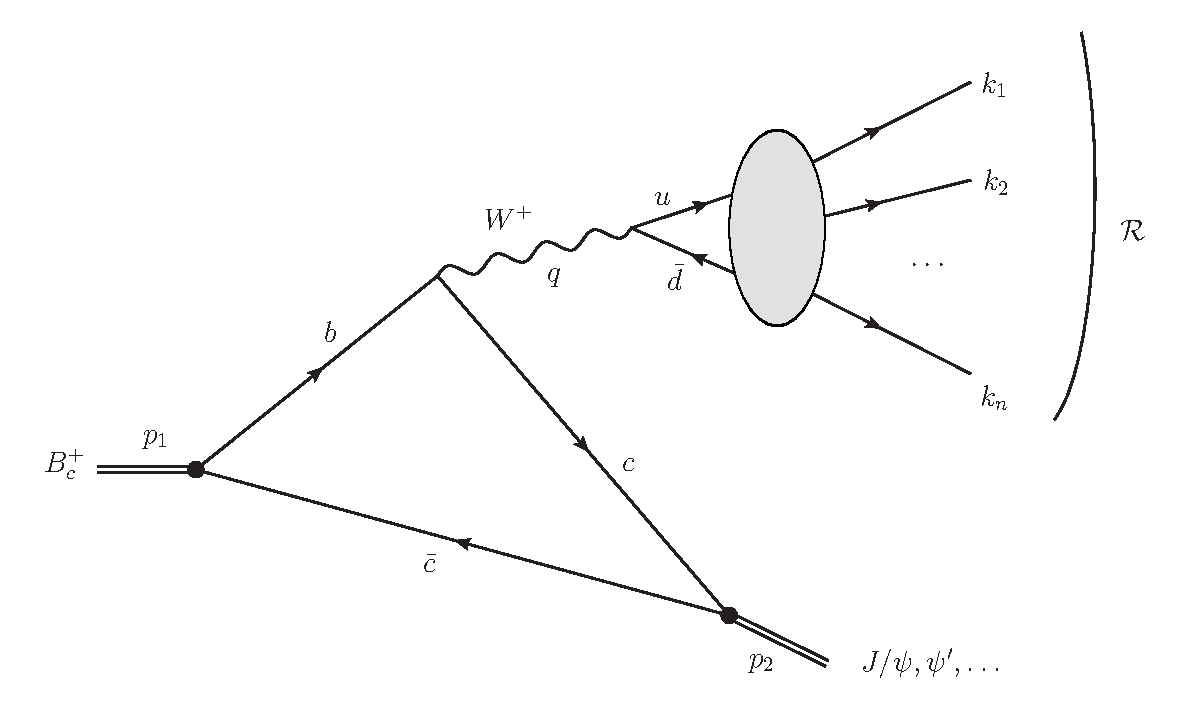
\includegraphics[width=0.5\columnwidth]{diags_BcCCW}
  \end{center}
      $$\M\left(B_c \to J/\psi + \R\right) = H^\mu \epsilon^{(\R)}_\mu$$
   where
   \begin{itemize}
   \item $H^\mu$ is the $B_c\to J/\psi W$ transition vertex
   \item $\epsilon^{(\R)}_\mu$ is effective  $W\to\R$ polarization vector
   \end{itemize}
The differential width is
$$
\frac{d\Gamma}{dq^2} \sim \frac{d\Gamma_T}{dq^2} \rho_T\left(q^2\right) + \frac{d\Gamma_L}{dq^2} \rho_L\left(q^2\right)
$$
\end{frame}


\begin{frame}
  \frametitle{$B_c \to J/\psi W$ transition}
\end{frame}

\begin{frame}
  \frametitle{$W\to R$ polarization vector}
\end{frame}

\subsection{$B_c\to J/\psi e\nu$}
\begin{frame}
  \frametitle{$B_c\to J/\psi e\nu$}
\end{frame}

\subsection{$B_c\to J/\psi \pi$, $B_c\to J/\psi \rho$}
\begin{frame}
  \frametitle{$B_c\to J/\psi \pi$, $B_c\to J/\psi \rho$}
\end{frame}

\subsection{$B_c\to J/\psi + n\pi$}
\begin{frame}
  \frametitle{$B_c\to J/\psi+ 2\pi$}
\end{frame}

\begin{frame}
  \frametitle{$B_c\to J/\psi + 3\pi$}
\end{frame}

\begin{frame}
  \frametitle{$B_c\to J/\psi +  5\pi$}
\end{frame}


\section{$B_c\to \chi_{cJ}+\R$}
\begin{frame}
  \frametitle{$B_c\to \chi_{cJ}+\R$}
\begin{center}
  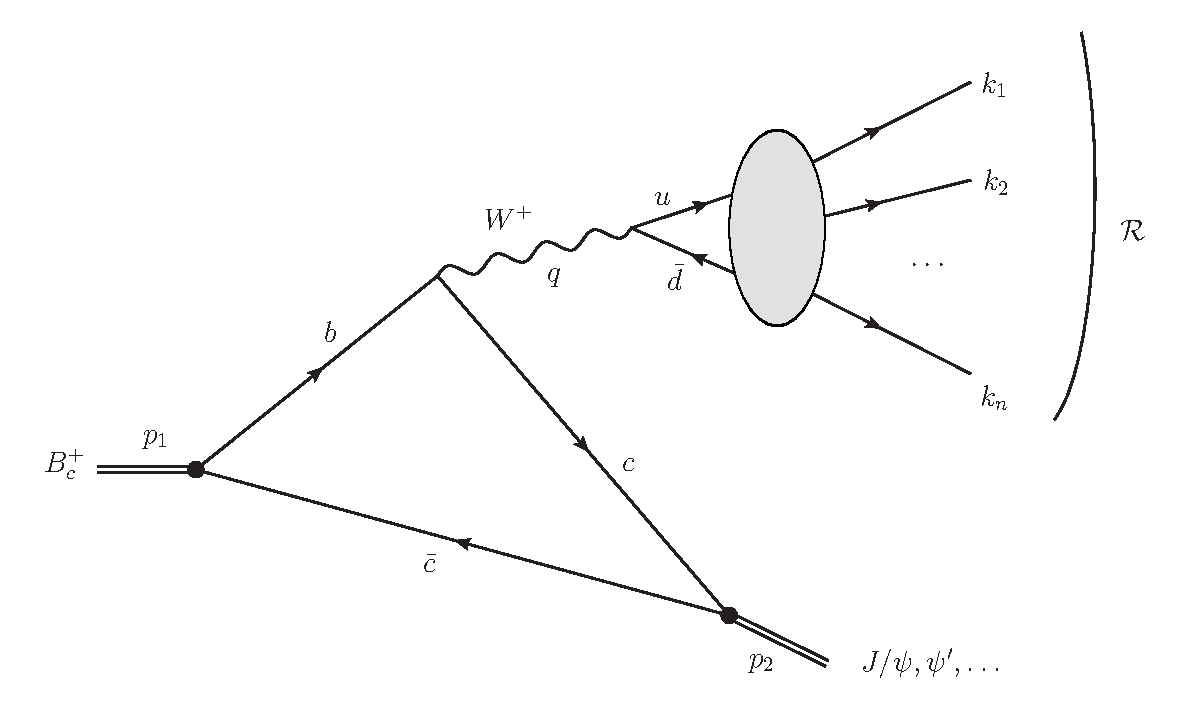
\includegraphics[width=0.5\columnwidth]{diags_BcCCW}
\end{center}
$$\M\left(B_c \to \chi_{cJ} + \R\right) = H^\mu \epsilon^{(\R)}_\mu$$
Form-factors of the $B_c\to \chi_{cJ}W$ transitions were considered in
\begin{itemize}
\item Ebert
\item Wang
\item Hernandez
\item etc.
\end{itemize}
\end{frame}

\subsection{$\chi_{c0}$}
\begin{frame}
  \frametitle{$\chi_{c0}$, Form Factors}
  $$
  H_\mu = f_{+}\left(q^2\right) \left(p_1+p_2\right)_\mu + f_{-}\left(q^2\right) \left(p_1-p_2\right)_\mu 
  $$
  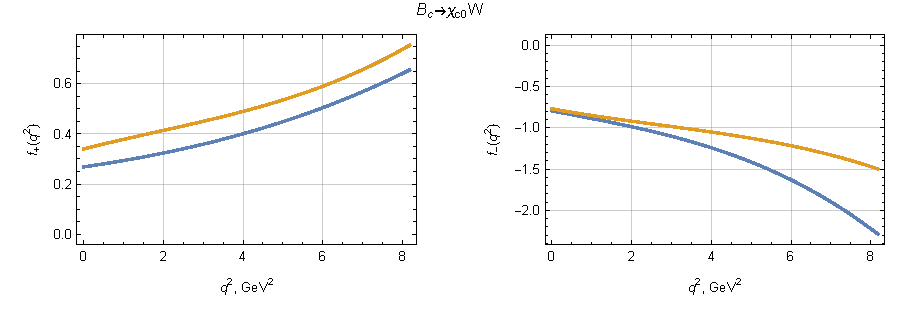
\includegraphics[width=0.9\textwidth]{figs/ff_chi_c0}

  $f_{-}(q^2)$ gives no contribution to most of the decays
  
  $f_{+}(q^2)$ are proportional to each other
\end{frame}

\begin{frame}
  \frametitle{$B_c \to \chi_{c0} e \nu$}
  \begin{center}
    \includegraphics[width=0.8\textwidth]{enu_chi_c0}
  \end{center}
  Branching fractions of semileptonic decays
  $$
  \begin{array}{c|cc}
 \text{None} & \text{[Ebert]} & \text{[Wang]} \\
\hline
 \chi _{\text{c0}} & 0.12 & 0.18 \\
  \end{array}
  $$
\end{frame}

\subsection{$\chi_{c1}$}
\begin{frame}
  \frametitle{$\chi_{c1}$, Form Factors}
  \begin{align*}
    \label{eq:1}
    H_\mu =& \frac{2i h_A(q^2)}{M_1+M_2}e_{\mu\nu\rho\sigma}\epsilon^\nu p_1^\rho p_2^\sigma
             + (M_1+M_2) h_{V_1}(q^2)\epsilon_\mu + \\
     & [h_{V_2}(q^2)p_{1\mu} + h_{V_3}(q^2)p_{2\mu}]\frac{\epsilon q}{M_1}
  \end{align*}
  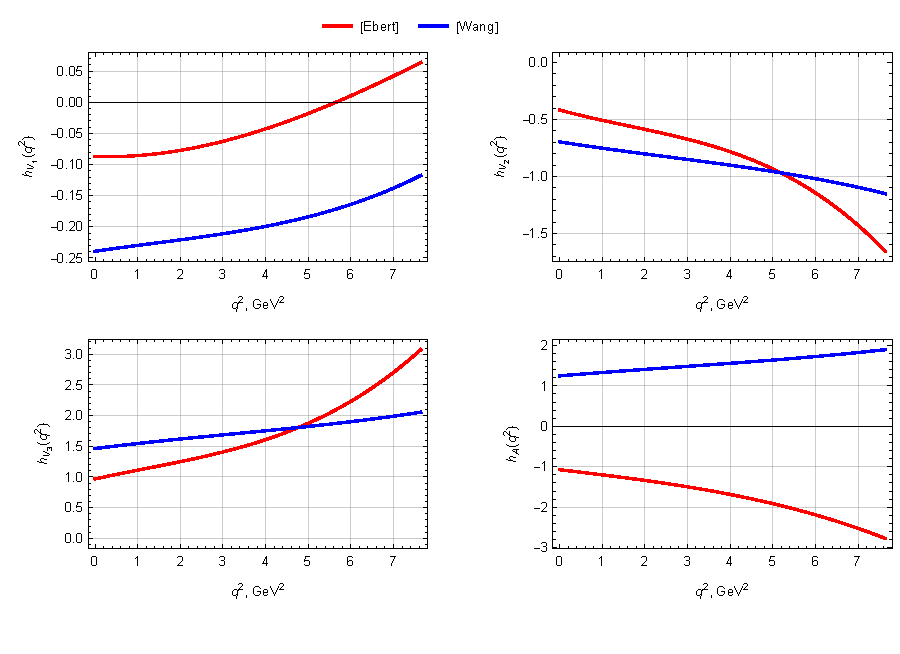
\includegraphics[width=0.9\textwidth]{figs/ff_chi_c1}
\end{frame}


\begin{frame}
  \frametitle{$B_c \to \chi_{c1} e \nu$}
  \begin{center}
    \includegraphics[width=0.8\textwidth]{enu_chi_c1}
  \end{center}
  Branching fractions of semileptonic decays
  $$
\begin{array}{c|cc}
 \text{None} & \text{[Ebert]} & \text{[Wang]} \\
\hline
 \chi _{\text{c1}} & 0.11 & 0.15 \\
\end{array}
$$
\end{frame}


\subsection{$\chi_{c2}$}
\begin{frame}
  \frametitle{$\chi_{c2}$, Form Factors}
  \begin{align*}
  H_\mu &=
\frac{2it_V(q^2)}{M_1+M_2} \epsilon^{\mu\nu\rho\sigma}\epsilon^*_{\nu\alpha}
          \frac{p_1^\alpha}{M_1}  p_1 p_1  
     +  (M_1+M_2)t_{A_1}(q^2)\epsilon^{*\mu\alpha}\frac{p_{1\alpha}}{M_1} +\\
&  [t_{A_2}(q^2)p_1^\mu+t_{A_3}(q^2)p_2^\mu]\epsilon^*_{\alpha\beta}
\frac{p_1^\alpha p_1^\beta}{M_1^2} , 
  \end{align*}

\begin{center}
  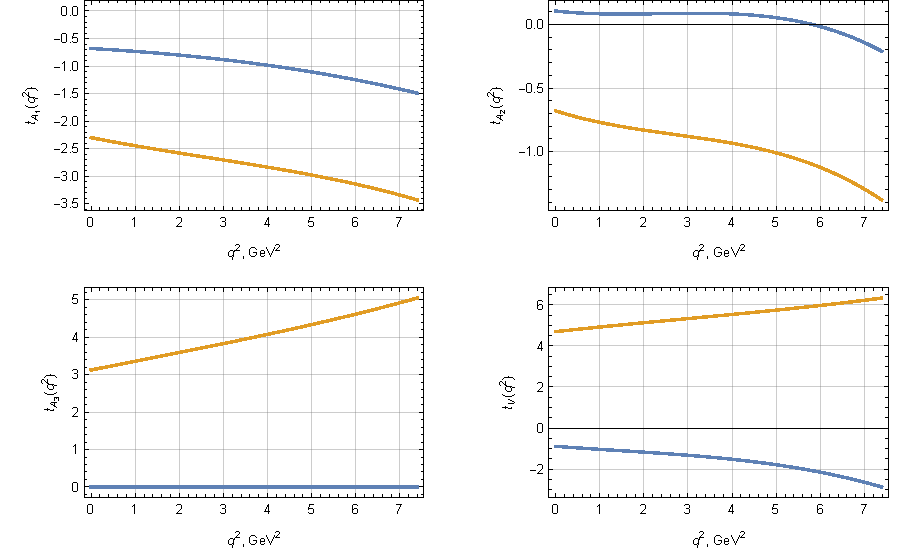
\includegraphics[width=0.7\textwidth]{figs/ff_chi_c2}
\end{center}
\end{frame}



  
\section{$B_c\to \chi_{cJ}+n\pi$}
\begin{frame}
  \frametitle{$B_c\to \chi_{cJ}+n\pi$}
\end{frame}

\section{EvtGen}
\begin{frame}
  \frametitle{EvtGen}
\end{frame}


\section{Conclusion}
\begin{frame}
  \frametitle{Conclusion}
\end{frame}


\end{document}
